% 引用tikz文档类
\documentclass[tikz]{standalone}

% 使用xcolor宏包并设置自定义颜色
\usepackage{xcolor}
\definecolor{DeepSkyBlue4}{RGB}{0,104,139}

% 引入中文环境,设定模式为plain,使用自定义字体设定
\usepackage[fontset=custom ,UTF8, scheme=plain]{ctex}

% 引入符号字体
\usepackage{fontawesome5}

% 设定tikz引用库
\usetikzlibrary{mindmap,shadows}

% 设定所有tikz图形中所用的字体为sans,对应自定义字体文件中的\setsansfont
\tikzset{every picture/.style={/utils/exec={\sffamily}}}

% 设定1级节点属性
\tikzstyle{level 1 concept}+=[
  % 每个节点旋转排列的间隔角度
  sibling angle=72,
  % 与上一层的节点的间距
  % level distance=40mm,
]

% 设置2级节点属性
\tikzstyle{level 2 concept}+=[
  % 每个节点旋转排列的间隔角度
  sibling angle=45,
  % 与上一层的节点的间距
  % level distance=20mm,
]

% 文档开始
\begin{document}
\begin{tikzpicture}[
    mindmap,
    % 设定所有图形的缩放比率,数字越大图形越小
    % scale=1.5,
    % transform shape,
    % 子节点采用圆形方式向外生长
    grow cyclic,
    % 所有节点增加阴影效果
    every node/.style={concept,circular drop shadow},
  ]
  \path[mindmap,concept color=teal,text=white]
  % font为字体设置,\fontsize{字号}{行间距},\selectfont必须有才会生效
  node[concept, font=\fontsize{30}{30}\selectfont] {\faHome}
    % 第一个子节点开始生长的角度
    [clockwise from=18]
    child[concept color=DeepSkyBlue4]{
      % font为字体设置,\fontsize{字号}{行间距},\selectfont必须有才会生效
      % shift={(72:2)}的意思是向72度方向漂移2cm
      node[concept, font=\fontsize{15}{15}\selectfont, shift={(72:2)}] {\faFolder\\src}
        % 第一个子节点开始生长的角度
        [clockwise from=11]
        child {node[concept] {\faLink\\awesome-cv.cls}}
        child {node[concept] {\faFileCode\\ctex-fontset-custom.def}}
        child {node[concept] {\faFileCode\\dukang.sty}}
        child {node[concept] {\faFileCode\\dukang-doc.tex}}
        child {node[concept] {\faFileCode\\main.tex}}
        child {node[concept] {\faFolder\\resource}}
        child {node[concept] {\faFolder\\dukang-doc}}
        child {node[concept] {\faFolder\\tex}}
    }
    child[concept color=teal!50] {node[concept] {awesome-cv.cls}}
    child[concept color=teal!80!green] {node[concept] {Makefile}}
    child[concept color=teal!50!pink]{node[concept] {icon.png}}
    child[concept color=teal!50!yellow] {node[concept] {README.md}};
\end{tikzpicture}
\end{document}
